
%% bare_conf.tex
%% V1.3
%% 2007/01/11
%% by Michael Shell
%% See:
%% http://www.michaelshell.org/
%% for current contact information.
%%
%% This is a skeleton file demonstrating the use of IEEEtran.cls
%% (requires IEEEtran.cls version 1.7 or later) with an IEEE conference paper.
%%
%% Support sites:
%% http://www.michaelshell.org/tex/ieeetran/
%% http://www.ctan.org/tex-archive/macros/latex/contrib/IEEEtran/
%% and
%% http://www.ieee.org/

%%*************************************************************************
%% Legal Notice:
%% This code is offered as-is without any warranty either expressed or
%% implied; without even the implied warranty of MERCHANTABILITY or
%% FITNESS FOR A PARTICULAR PURPOSE! 
%% User assumes all risk.
%% In no event shall IEEE or any contributor to this code be liable for
%% any damages or losses, including, but not limited to, incidental,
%% consequential, or any other damages, resulting from the use or misuse
%% of any information contained here.
%%
%% All comments are the opinions of their respective authors and are not
%% necessarily endorsed by the IEEE.
%%
%% This work is distributed under the LaTeX Project Public License (LPPL)
%% ( http://www.latex-project.org/ ) version 1.3, and may be freely used,
%% distributed and modified. A copy of the LPPL, version 1.3, is included
%% in the base LaTeX documentation of all distributions of LaTeX released
%% 2003/12/01 or later.
%% Retain all contribution notices and credits.
%% ** Modified files should be clearly indicated as such, including  **
%% ** renaming them and changing author support contact information. **
%%
%% File list of work: IEEEtran.cls, IEEEtran_HOWTO.pdf, bare_adv.tex,
%%                    bare_conf.tex, bare_jrnl.tex, bare_jrnl_compsoc.tex
%%*************************************************************************

% *** Authors should verify (and, if needed, correct) their LaTeX system  ***
% *** with the testflow diagnostic prior to trusting their LaTeX platform ***
% *** with production work. IEEE's font choices can trigger bugs that do  ***
% *** not appear when using other class files.                            ***
% The testflow support page is at:
% http://www.michaelshell.org/tex/testflow/



% Note that the a4paper option is mainly intended so that authors in
% countries using A4 can easily print to A4 and see how their papers will
% look in print - the typesetting of the document will not typically be
% affected with changes in paper size (but the bottom and side margins will).
% Use the testflow package mentioned above to verify correct handling of
% both paper sizes by the user's LaTeX system.
%
% Also note that the "draftcls" or "draftclsnofoot", not "draft", option
% should be used if it is desired that the figures are to be displayed in
% draft mode.
%
\documentclass[conference]{include/IEEEtran}
% Add the compsoc option for Computer Society conferences.
%
% If IEEEtran.cls has not been installed into the LaTeX system files,
% manually specify the path to it like:
% \documentclass[conference]{../sty/IEEEtran}



\usepackage{cite}
\usepackage[pdftex]{graphicx}

\def\xcolorversion{2.00}
\def\xkeyvalversion{1.8}
\usepackage[version=0.96]{pgf}
\usepackage{tikz}
\usetikzlibrary{arrows,shapes,snakes,automata,backgrounds,petri}


% *** SPECIALIZED LIST PACKAGES ***
%
%\usepackage{algorithmic}
% algorithmic.sty was written by Peter Williams and Rogerio Brito.
% This package provides an algorithmic environment fo describing algorithms.
% You can use the algorithmic environment in-text or within a figure
% environment to provide for a floating algorithm. Do NOT use the algorithm
% floating environment provided by algorithm.sty (by the same authors) or
% algorithm2e.sty (by Christophe Fiorio) as IEEE does not use dedicated
% algorithm float types and packages that provide these will not provide
% correct IEEE style captions. The latest version and documentation of
% algorithmic.sty can be obtained at:
% http://www.ctan.org/tex-archive/macros/latex/contrib/algorithms/
% There is also a support site at:
% http://algorithms.berlios.de/index.html
% Also of interest may be the (relatively newer and more customizable)
% algorithmicx.sty package by Szasz Janos:
% http://www.ctan.org/tex-archive/macros/latex/contrib/algorithmicx/


\usepackage[caption=false,font=footnotesize]{subfig}


% *** FLOAT PACKAGES ***
%
\usepackage{fixltx2e}
% fixltx2e, the successor to the earlier fix2col.sty, was written by
% Frank Mittelbach and David Carlisle. This package corrects a few problems
% in the LaTeX2e kernel, the most notable of which is that in current
% LaTeX2e releases, the ordering of single and double column floats is not
% guaranteed to be preserved. Thus, an unpatched LaTeX2e can allow a
% single column figure to be placed prior to an earlier double column
% figure. The latest version and documentation can be found at:
% http://www.ctan.org/tex-archive/macros/latex/base/






% *** PDF, URL AND HYPERLINK PACKAGES ***
%
%\usepackage{url}
% url.sty was written by Donald Arseneau. It provides better support for
% handling and breaking URLs. url.sty is already installed on most LaTeX
% systems. The latest version can be obtained at:
% http://www.ctan.org/tex-archive/macros/latex/contrib/misc/
% Read the url.sty source comments for usage information. Basically,
% \url{my_url_here}.





% *** Do not adjust lengths that control margins, column widths, etc. ***
% *** Do not use packages that alter fonts (such as pslatex).         ***
% There should be no need to do such things with IEEEtran.cls V1.6 and later.
% (Unless specifically asked to do so by the journal or conference you plan
% to submit to, of course. )


% correct bad hyphenation here
\hyphenation{}


\begin{document}
%
% paper title
% can use linebreaks \\ within to get better formatting as desired
\title{Curiosity-driven Exploration of Skill Hierarchies}


% author names and affiliations
% use a multiple column layout for up to three different
% affiliations
\author{\IEEEauthorblockN{S\'ebastien Forestier}
\IEEEauthorblockA{INRIA Bordeaux Sud-Ouest\\
Bordeaux, France\\
Email: sebastien.forestier@inria.fr}
\and
\IEEEauthorblockN{Pierre-Yves Oudeyer}
\IEEEauthorblockA{INRIA Bordeaux Sud-Ouest\\
Bordeaux, France\\
Email: pierre-yves.oudeyer@inria.fr}}

% conference papers do not typically use \thanks and this command
% is locked out in conference mode. If really needed, such as for
% the acknowledgment of grants, issue a \IEEEoverridecommandlockouts
% after \documentclass

% for over three affiliations, or if they all won't fit within the width
% of the page, use this alternative format:
% 
%\author{\IEEEauthorblockN{Michael Shell\IEEEauthorrefmark{1},
%Homer Simpson\IEEEauthorrefmark{2},
%James Kirk\IEEEauthorrefmark{3}, 
%Montgomery Scott\IEEEauthorrefmark{3} and
%Eldon Tyrell\IEEEauthorrefmark{4}}
%\IEEEauthorblockA{\IEEEauthorrefmark{1}School of Electrical and Computer Engineering\\
%Georgia Institute of Technology,
%Atlanta, Georgia 30332--0250\\ Email: see http://www.michaelshell.org/contact.html}
%\IEEEauthorblockA{\IEEEauthorrefmark{2}Twentieth Century Fox, Springfield, USA\\
%Email: homer@thesimpsons.com}
%\IEEEauthorblockA{\IEEEauthorrefmark{3}Starfleet Academy, San Francisco, California 96678-2391\\
%Telephone: (800) 555--1212, Fax: (888) 555--1212}
%\IEEEauthorblockA{\IEEEauthorrefmark{4}Tyrell Inc., 123 Replicant Street, Los Angeles, California 90210--4321}}




% use for special paper notices
%\IEEEspecialpapernotice{(Invited Paper)}




% make the title area
\maketitle


\begin{abstract}
%\boldmath
The abstract goes here.
\end{abstract}
% IEEEtran.cls defaults to using nonbold math in the Abstract.
% This preserves the distinction between vectors and scalars. However,
% if the conference you are submitting to favors bold math in the abstract,
% then you can use LaTeX's standard command \boldmath at the very start
% of the abstract to achieve this. Many IEEE journals/conferences frown on
% math in the abstract anyway.

% no keywords




% For peer review papers, you can put extra information on the cover
% page as needed:
% \ifCLASSOPTIONpeerreview
% \begin{center} \bfseries EDICS Category: 3-BBND \end{center}
% \fi
%
% For peerreview papers, this IEEEtran command inserts a page break and
% creates the second title. It will be ignored for other modes.
\IEEEpeerreviewmaketitle



\section{Introduction}

	
	The study of the control of manipulation actions in humans has revealed a modular representation of actions 
	either in the cerebral cortex and in the spinal 
	cord with compositionality: an infinite number of movements can be expressed through combination of simple primitives, 
	and generalization: certain neurons (higher 
	in the hierarchy) can represent actions independently of the effectors used \cite{cangelosi2010integration}.
	
	The same idea holds for language expressiveness which is based on syntactic hierarchical combinations 
	on a vocabulary, that open infinite semantic possibilities. 
	Greenfield has also argued that this parallel between manipulation and language compositionality can be found in the human ontegenic development
	with combinatorial steps for manipulation and syntax acquired approximately at the same period and in the same order \cite{green}. 
	Also, the author explains that the development of the neural substrates for language and tool use could be an ontogenic homology as first of all
	the same neural computations for hierarchical combinations and their semantics should take place for both modalities, and furthermore 
	experiments with Broca's and Wernicke's aphasics show that hierarchical organization for language and manipulation is linked. 
	Broca's aphasics, who have less syntactic organization of speech were shown to also have problems of representation of the hierarchical organization
	of constructions with blocks, whereas Wernicke's aphasics, whose syntax is normal but speech semantics is impaired, succeed in representing such objects 
	hierarchies. 
	
	Functional MRI experiments by Higuchi et al. have shown that the human's neural substrates for tool use and language is indeed shared in 
	the dorsal BA44 Broca's area \cite{higuchi}, which gives evidence for the similar neural computations used. 
	They furthermore argue that these results supports the hypothesis that tool use have appeared first in primate evolution in F5 area,
	and then the language has developed in humans reusing part of tool use and manipulation neural substrates in human's Broca area, homolog of primate's F5.

	Like a developing child, a developmental robot will have to incrementally explore skills that add up to the hierarchy of previously learned skills 
	throughout its life, with a constraint being the cost and time of experimentation. 
	We will seek to define curiosity-driven hierarchical learning architectures 
	that could reuse the sensorimotor contingencies previously learned and to combine them 
	to explore more efficiently new complex sensorimotor models. 
		
	\subsection{Goal of the study}
			
		\begin{itemize}
			\item Exploring in a structured hierarchy is more efficient than directly from $M$ to $S$.
			\item Which task should I explore now ?
			\item How to choose between different means to explore a given space ? 
			\item How can high-level tasks guide the exploration of lower-level ones ?
			\item How can the system cope with perturbations on some of the forward models ?		
		\end{itemize}

		
	%
	
	\subsection{Related work}
		\cite{ugur2014, ugur2015}.

		Different computational models have the possibility to learn skill hierarchies. 
		In finite environments represented by a factored Markov Decision Process \cite{vig}, an intrinsic motivation towards actions 
		maximizing Dynamic Bayesian Networks' structure has been shown to allow the learning of the environment's structure.
		
		In continuous environments but with discrete actions, Metzen et al. \cite{metzen2013} use the framework of options \cite{sutton1999between} 
		to learn skill hierarchies. 
		An intrinsic motivation rewards positively the novelty of the states encountered and negatively the prediction error of the learned skill model.
		
		The model from Fabisch et al. \cite{fabisch2014active} learns in a setting with a discrete task space (called contexts).
		It uses an intrinsic motivation for learning progress, and a Multi-Armed Bandit algorithm (D-UCB) to choose on which context the agent should train for.
		The Upper Confidence Bound algorithm chooses between contexts given their estimated learning progress and the uncertainty of these estimations
		by picking the context with the maximum upper confidence bound.
		In other words, it maximizes the expected reward plus something related to the uncertainty associated with it, selecting either contexts with 
		certain high rewards or ones with uncertain poor reward.
		This algorithm embeds directly a solution the exploration-exploitation trade-off problem as it represents the exploitation 
		of knowledge by the expected progress and the exploration of other solutions by the uncertainty bonus. 
		This algorithm supposes a stationary learning progress on each context so the authors use an adaptation 
		(D-UCB, \cite{kocsis2006discounted}) to encompass non-stationary learning progress.
		% Sliding Window UCB: \cite{garivier2011upper}
		
		In a fully continuous setting, Mugan et al. \cite{mugan} have developed an algorithm that first learns a qualitative representation of environment states
		and actions in order to then learn the structure of Dynamic Bayesian Networks representing the temporal contingencies of those states and actions.
		In order to choose which action to practice, the authors use the IAC \cite{oudeyer_intrinsic_2007} where the agent 
		is intrinsically motivated to choose actions that are estimated to yield high prediction error progress.
		
		Here, we will rely more specifically on the SAGG-RIAC architecture \cite{baranes_active_2013}.
		This architecture learns a single mapping between continuous motor and sensori (or task) 
		spaces with a competence-based intrinsic motivation. 
		In our hierarchy of sensorimotor models, each model will be explored using the SAGG-RIAC procedure, but it could be replaced by another one 
		without changing the mechanisms to learn the hierarchy that will be assessed.

	%
%


\section{Environment}

	We simulate a 2D robotic arm using tools to push an object in its environment with the help of an experienced pair. 
	The agent can either try to push objects into boxes on its own, or produce a vocal signal that might engage the experienced pair to help move the object to reach a box.
	
	The environment is designed such that each box is more easily reached by one different mean.
	Box 1 is best reached with the small stick, box 2 with the long stick, and box 3 with the small stick and the help of the pair.
	
	An iteration consists of the evaluation of a motor command given by the agent which gives
	sensory information back to him, and 
	finally the environment is resetted to its intial state.
	
	\begin{figure}[!t]
		\centering
		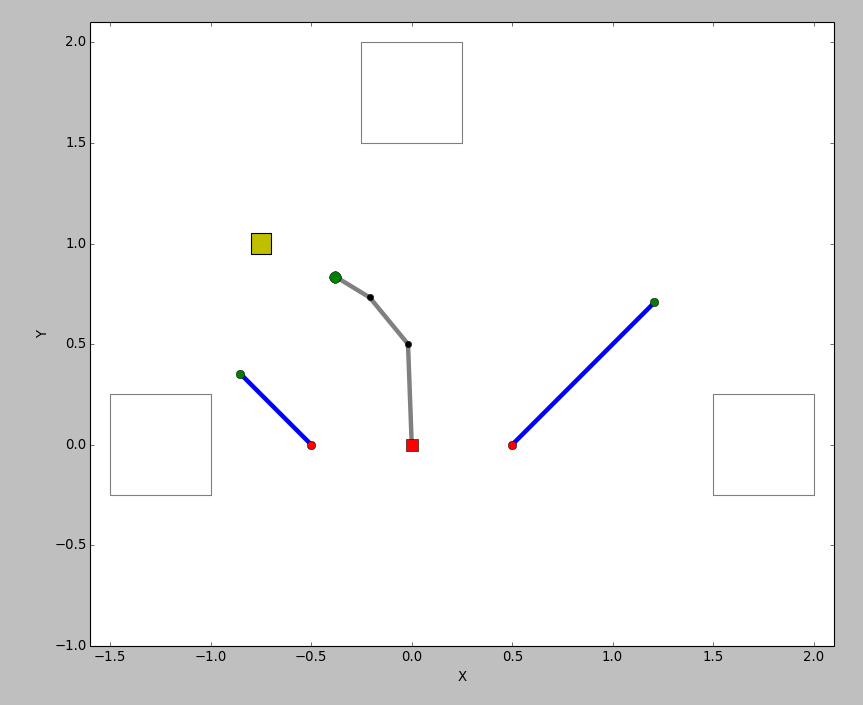
\includegraphics[width=8cm]{./include/tools.png}
		\caption{Play Environment}
		\label{env}
	\end{figure}
		
	The next sections precisely describe the different items of the environment and their interactions.	
	See Fig. \ref{env} for an exemple of the state of the environment. 
	

	\subsection{Robotic arm}
	
		The 2D robotic arm has 3 joints plus a gripper located at the end-effector.
		Each joint can rotate from $-\pi~rad$ to $\pi~rad$ around its initial position, mapped to a standard interval of $[-1,1]$.
		The length of the 3 parts of the arm are $0.5$, $0.3$ and $0.2$ so the total length of the arm is $1$ unit.
		The initial position of the arm is vertical with each joint at $0~rad$ and its base is fixed at position $[0, 0]$.
		The gripper $g$ has 2 possible positions: \textit{open} ($g \geq 0$) and \textit{closed} ($g < 0$) and its initial position is \textit{open} (with $g = 0$).
		The robotic arm thus has 4 degrees of freedom represented by a vector in $[-1,1]^4$.
		A trajectory of the arm will be represented as a sequence of such vectors.
	
	%
	
		
	\subsection{Objects and tools}
		
		A yellow squared object can be moved into one of the 3 fixed squared boxes. 
		The initial position of the yellow square is $(-0.75, 1)$ and is thus unreachable with directly with the gripper.
		One of 2 sticks can be grasped in order to reach the object.
		A small stick of length $0.5$ is located on the left of the arm, with initial position $(-0.5, 0)$ and initial angle $\frac{3\pi}{4}$ from the horizontal line.
		A long stick of length $1.$ is located on the right of the arm, with initial position $(0.5, 0)$ and initial angle $\frac{\pi}{4}$ from the horizontal line as in Fig. \ref{env}.
		
		If the gripper closes near the end of one of the sticks (closer than $0.2$), it is considered grasped and will follow the gripper's position and the angle (with some noise) of the arm's last part until the gripper opens.
		The grasped stick will have its angle equal to arm's last part plus a gaussian noise (of size $0.02$ for the small sitck and $0.1$ for the long one), updated at each step of the movement.
		
		Similarly, if the other end of a stick reaches the yellow squared object (within $0.25$), the object will follow the end of the stick.
		Three boxes are fixed at positions $(-1.25, 0)$, $(0, 1.75)$ and $(-1.75, 0)$ and have size $0.5$.
		At the end of the trial, the object is considered to be in one of the box if its center is in the box.
	
	%
	
	\subsection{Help from an experienced pair}
	
		A pair sitting at the right of the robot will help him put the yellow square into the closer box.
		It will wait for the robot to move the object on its own, and if the robot also produces the good vocal signal, will move the object to the closest box.
		
		However, as the long stick is long enough to reach the any of the 3 boxes but not the small one, the pair will help the robot only when it will use the small stick.
		Also, as the pair is sitting on the right side of the robot, it will be unable to help reach box 1 (on the left).
		The pair will help reach box 2 (on the front) but with a bad precision as it is far, and box 3 (on the right) with a good precision.
		The pair will put the object at the center of box 2 (with a gaussian noise of size $0.2$ on x and y dimensions thus missing the box quite often), 
		only if the object is located near box 2 at a distance from the base of the arm greater than $1.$ and an angle from the horizontal line between $45°$ and $105°$.
		If the angle is between $-15°$ and $45°$, then the pair moves it towards the center of box 3 with a gaussian noise of size $0.05$, thus rarely missing the box.
		
		We simulate a simple vocal signal controled by pitch and intensity between $-1$ and $1$.
		The pair will engage in helping the robot only if pitch and intensity were sufficiently high ($>0.$).
	%
	
	\subsection{Motor control}
	
		We use Dynamical Movement Primitive \cite{ijspeert_dynamical_2013} to control the arm's movement as this framework permits the production of a diversity of arm's trajectories with few parameters.
		Each of the 4 arm's degree of freedom (DOF) is controlled by a DMP with a starting and a goal position equal to the rest position of the joint.
		Each DMP is parameterized by one weight on each of 3 basis functions whose centers are distributed homogeneously throughout the movement.
		The weights are bounded in the interval $[-200,200]$ (mapped to the standard interval $[-1,1]$) which allow each joint to cover its standard interval $[-1,1]$ during the movement.
		Each DMP outputs a series of $50$ positions that represents a sampling of the trajectory of one joint during the movement.
	
		The arm's movement is thus parameterized by $12$ weights, and the static vocal signal by $2$ weights.
		Let $M_a$ be the $12D$ space of arm's commands $[-1,1]^{12}$, $M_v$ be the $2D$ vocal space, and $M$ the $14D$ global motor space.
	
	%
	
	\subsection{Sensory feedback}
	
		At the end of the movement, the robot gets sensory feedback from the different items of the environment.
		It gets the trajectory of its hand and gripper, whether the vocal signal engaged the pair or not, the trajectory of the end of the sticks, 
		the end position of the object, and whether the object is in each box and at which distance.
	
		The trajectory of the hand and of the end point of the sticks is the sequence of x and y positions at different time points: steps $12$, $25$, $37$ during the movement of $50$ steps.
		The trajectory of the gripper is a sequence of $1$ or $-1$ depending whether the gripper is open or not.
		The pair understanding of the vocal signal is represented as $1$ if intensity and pitch were correct, $-1$ otherwise.
		For each box, the robot receives a $1$ if the object was in the box, and $0$ otherwise, plus the distance between the end position of the object and the center of the box.
		 
		The sensory information thus contains $6$ dimensions for the trajectory of the hand, $1$ for the pair help, $6$ for the trajectory of the end of each stick, $2$ for the end position of the object, and $2$ for each box.
		The total sensory space has $44$ dimensions.
		
	%
	
	
%
	
\section{Random Goal Babbling}


	
%


\section{Hierarchically structured exploration}


	\begin{figure}[!t]
		\center
		
% H2
\begin{tikzpicture}[node distance=1cm,>=stealth',bend angle=45,auto]

	\tikzstyle{dom}   = [ellipse, thick, draw=black!75, fill=blue!20,  minimum height=4mm, minimum width=4mm]
	\tikzstyle{prim dom}   = [dom,  minimum height=5mm, minimum width=5mm,  fill=green!20]
	\tikzstyle{mod} = [rectangle, thick, draw=black!75, fill=black!20, minimum size=3mm]

	\begin{scope}
		\scriptsize
		\node [prim dom, label=below:$12$D] (pd1) {$Arm$};

		\node [mod, label=above:$Model_1$] (m1) [right of=pd1, xshift=-0.1cm] {$1$}
		edge [pre]                  (pd1);

		\node [dom, label=below:$9$D] (d1) [right of=m1] {$Hand$}
		edge [pre]                (m1);
		
		\node [mod] (m3) [right of=d1, xshift=-0.1cm,yshift=0.4cm] {$2$}
		edge [pre]                  (d1);
		
		\node [dom, label=below:$6$D] (d3) [right of=m3, xshift=-0.1cm,yshift=0.4cm] {$Stick_1$}
		edge [pre]                (m3);
		
		\node [mod] (m6) [right of=d1, xshift=-0.1cm,yshift=-0.4cm] {$5$}
		edge [pre]                  (d1);
		
		\node [dom, label=above:$6$D] (d6) [right of=m6, xshift=-0.1cm,yshift=-0.4cm] {$Stick_2$}
		edge [pre]                (m6);
		
		\node [mod] (m7) [right of=d6,yshift=0.2cm] {$6$}
		edge [pre]                  (d6);
		
		\node [mod] (m4) [right of=d3,yshift=-0.2cm] {$3$}
		edge [pre]                  (d3);
		
		\node [dom, label=below:$2$D] (d4) [right of=m4, xshift=-0.3cm,yshift=-0.6cm] {$Object$}
		edge [pre]                (m4)
		edge [pre]                (m7);
		
		\node [mod] (m5) [right of=d4] {$4$}
		edge [pre]                  (d4);
		
		\node [dom, label=below:$2$D] (d5) [right of=m5] {$Boxes$}
		edge [pre]                (m5);
		
		
	\end{scope}
	\begin{pgfonlayer}{background}
		\filldraw [line width=2mm,black!10]
		(d3.north  -| d5.east)  rectangle (d6.south  -| pd1.west);
	\end{pgfonlayer}
\end{tikzpicture}

		\caption{H1}
		\label{H1}					
	\end{figure}
	
	
	% Experiment 1
	\subsection{Experiment 1: Methods}		
				
		\begin{itemize}
			\item Idea: to compare our simplest algorithm (explore the module with higher progress) in a realistic setting (Hierarchy (a) of Fig. \ref{Hierarchies}) to the control condition where a sensorimotor model is learned
					directly from the whole motor space $M$ to the whole sensori space $S$.
			
			\item Conditions: Hierarchy (a) vs $M \rightarrow S$, Motor Babbling vs SAGG-Random
			
			\item Features: MAB on all modules, NN, No TDD.
			
			\item Measures: exploration of intermediate spaces (hands, tools), exploration of top spaces (objects). Competence to reach random goals in reachable parts of intermediate and top spaces. 
					Statistics on multiple runs to see regularity/diversity in developmental trajectories.
		\end{itemize}
		
	%
			
	\subsection{Experiment 1: Results}
	
		\begin{figure*}[!t]
			\centering
			\subfloat[Competences]{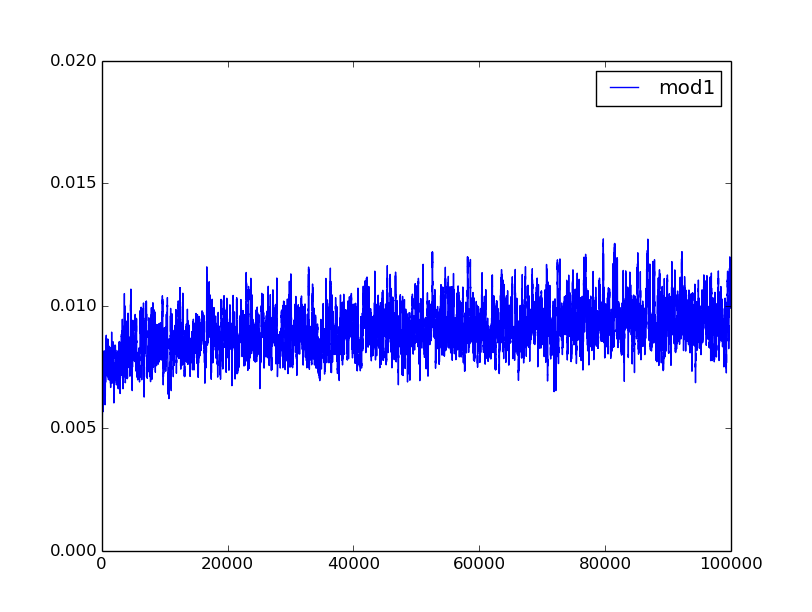
\includegraphics[width=6cm]{./include/H0-GB-log6-competences.png}}
			\subfloat[Interests]{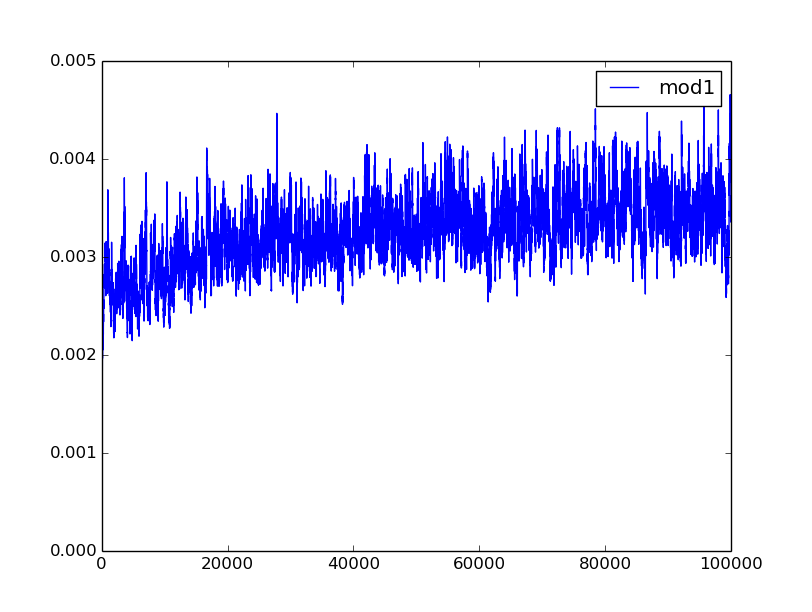
\includegraphics[width=6cm]{./include/H0-GB-log6-interests.png}}
			\subfloat[Events]{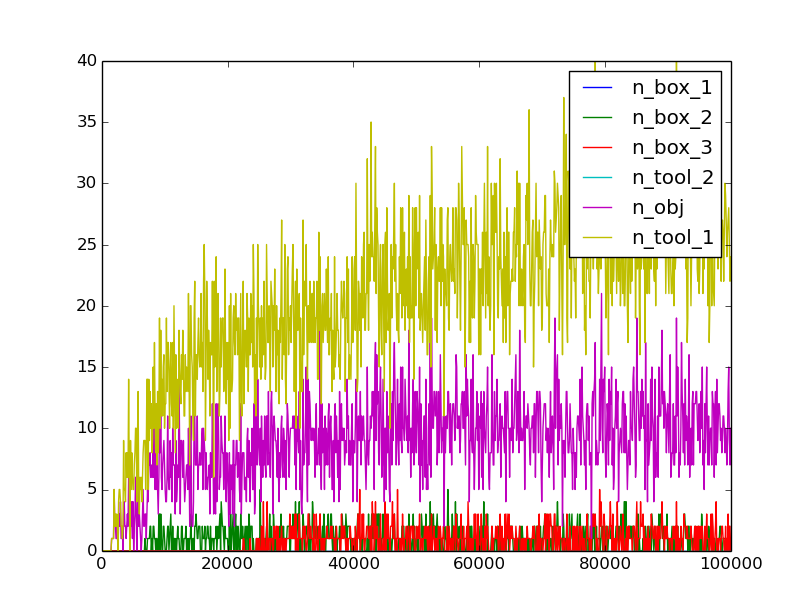
\includegraphics[width=6cm]{./include/H0-GB-log6-events.png}}
			\caption{Competences, interests and events using H0 with Random Goal Babbling}
			\label{resH0GB}
		\end{figure*}
		
		\begin{figure*}[!t]
			\centering
			\subfloat[Competences]{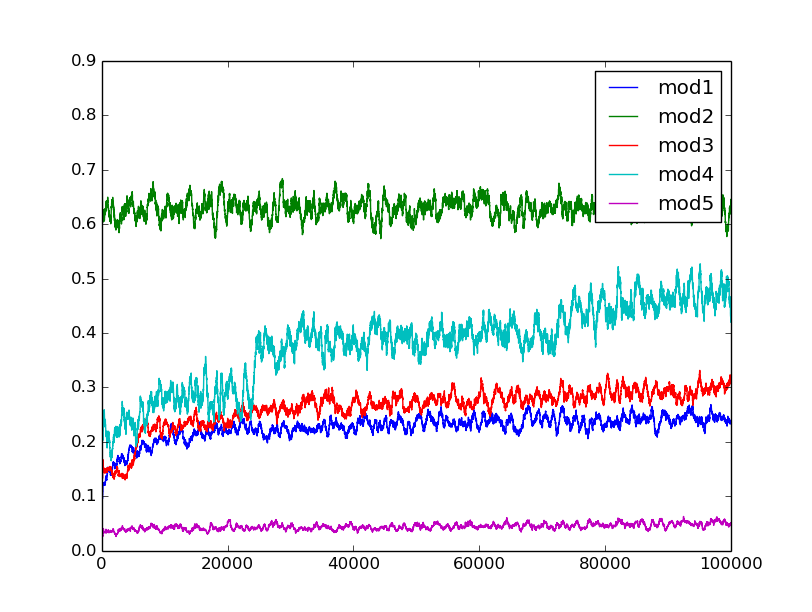
\includegraphics[width=6cm]{./include/H1-GB-log5-competences.png}}
			\subfloat[Interests]{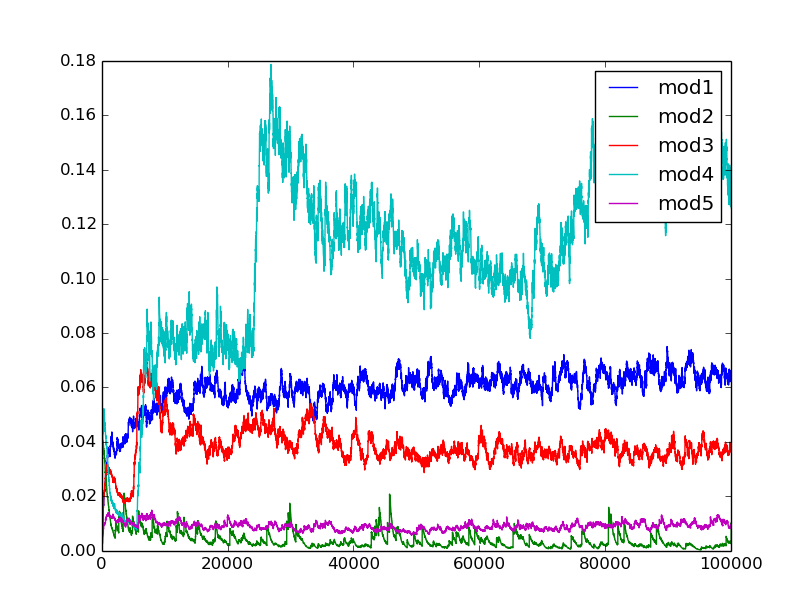
\includegraphics[width=6cm]{./include/H1-GB-log5-interests.png}}
			\subfloat[Events]{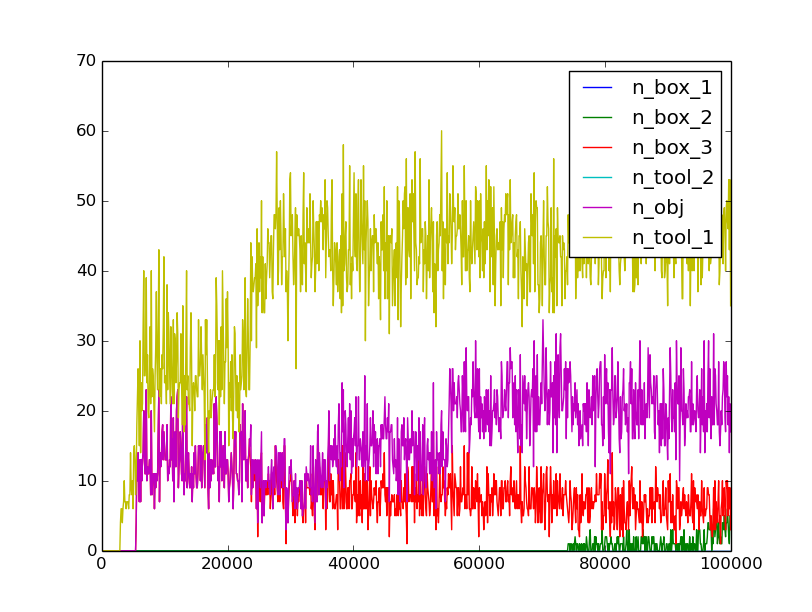
\includegraphics[width=6cm]{./include/H1-GB-log5-events.png}}
			\caption{Competences, interests and events using H1 with Random Goal Babbling}
			\label{resH1GB}
		\end{figure*}
		
		\begin{figure*}[!t]
			\centering
			\subfloat[Tool]{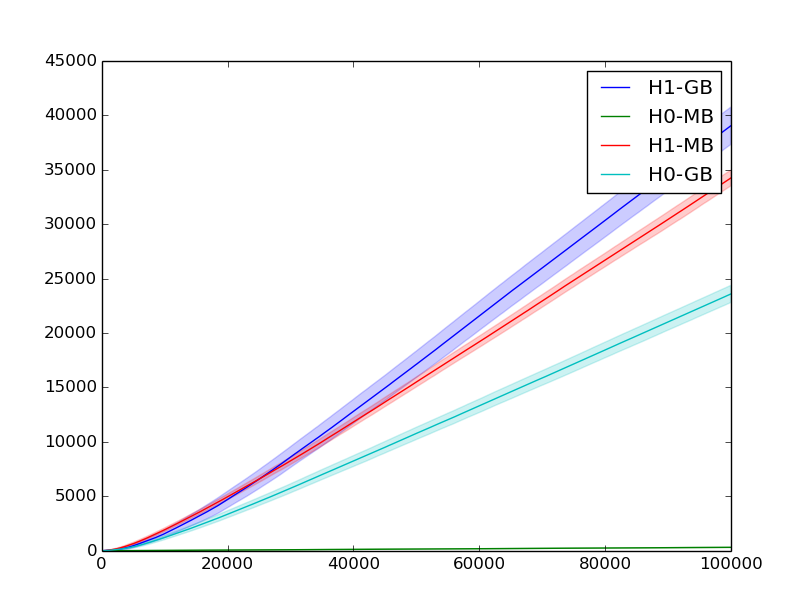
\includegraphics[width=6cm]{./include/xp1-n_tool_1.png}}
			\subfloat[Object]{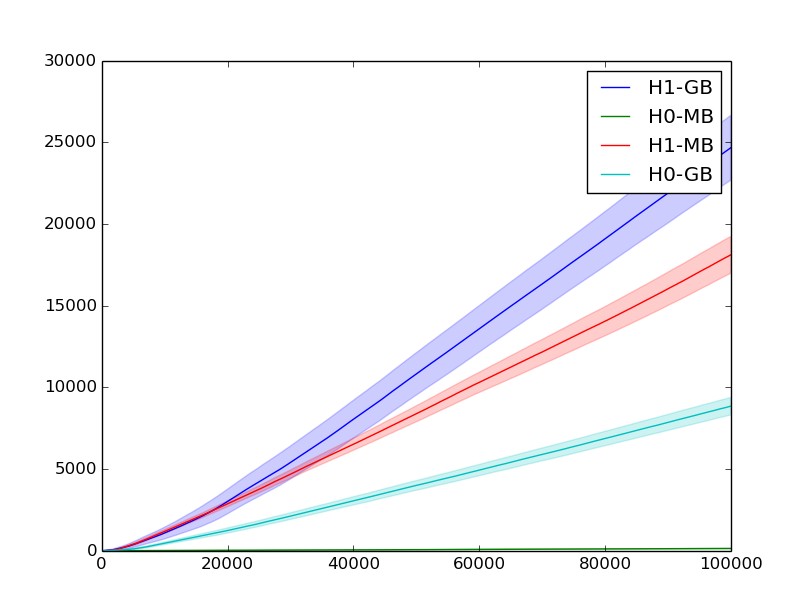
\includegraphics[width=6cm]{./include/xp1-n_obj.png}}
			\subfloat[Box 1]{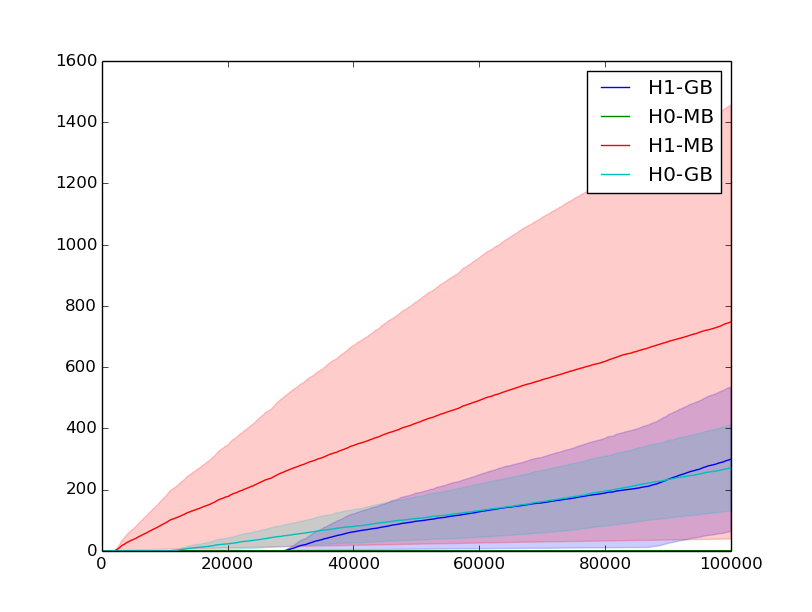
\includegraphics[width=6cm]{./include/xp1-n_box_1.png}}\\
			\subfloat[Box 2]{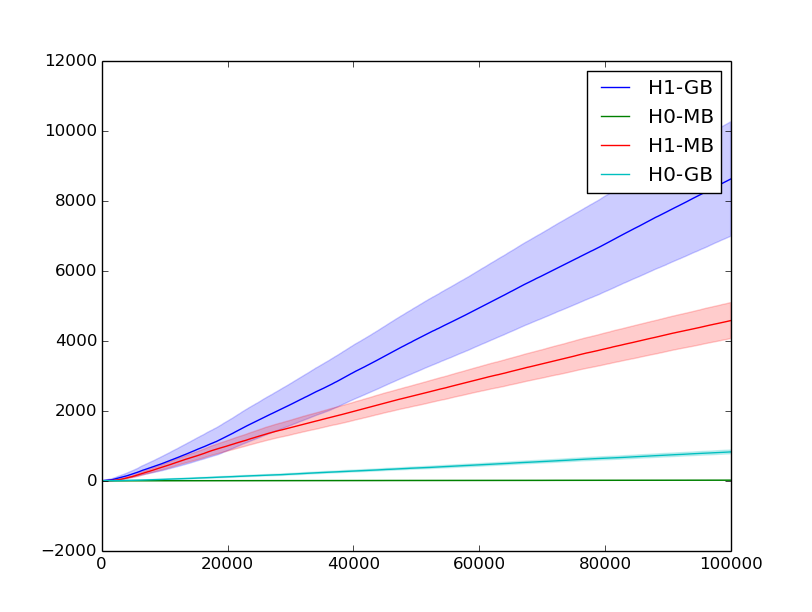
\includegraphics[width=6cm]{./include/xp1-n_box_2.png}}
			\subfloat[Box 3]{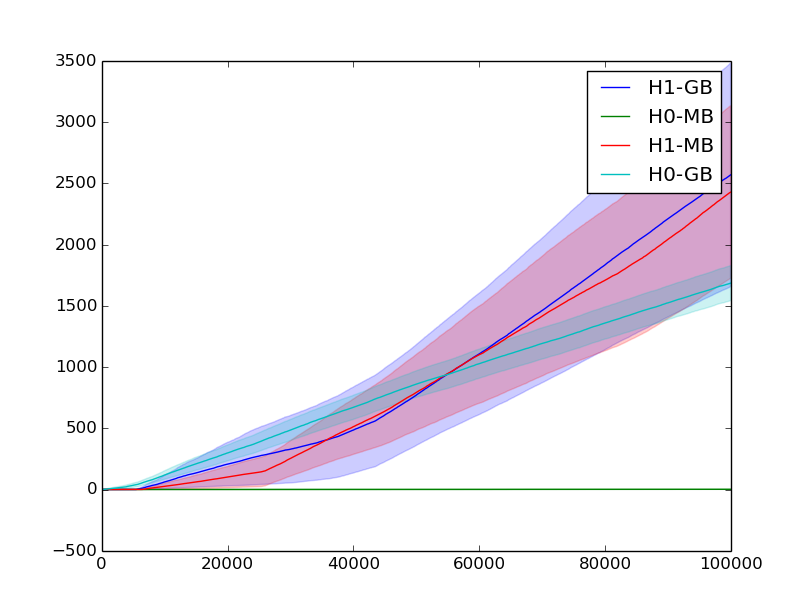
\includegraphics[width=6cm]{./include/xp1-n_box_3.png}}
			\caption{Number of touch of tool, object and boxes for each 100 iterations' bin.}
			\label{res_xp1_events}
		\end{figure*}
		
		
		See Fig. \ref{resH0GB}, \ref{resH1GB} and \ref{res_xp1_events}.
		
	%
	
	\subsection{Experiment 1: Discussion}	
	
	%

%
	
\section{Choice of module to explore}


	
	% Experiment 2
	\subsection{Experiment 2: Methods}	
		
		\begin{itemize}
			\item Idea: to compare the different possibilities to choose the module to explore in the hierarchy: maximizing the progress, maximizing with a bias towards lower-level modules, or use ZPDES,
					with the same hierarchy (a) of Fig. \ref{Hierarchies}.
			
			\item Conditions: Random module, MAB on all modules, MAB with bias, ZPDES.
			
			\item Features: Hierarchy (a), SAGG-Random, NN, No TDD.
			
			\item Measures: exploration of intermediate spaces (hands, tools), exploration of top spaces (objects). Competence to reach random goals in reachable parts of intermediate and top spaces. 
					Statistics on multiple runs to see regularity/diversity in developmental trajectories.
		\end{itemize}
		
	%
		
	
	\subsection{Experiment 2: Results}

		
	%
	
	\subsection{Experiment 2: Discussion}	
	
	%

%
	
\section{Choice of tool to use}

	\begin{figure}[!t]
		\center
		
% H2
\begin{tikzpicture}[node distance=1.cm,>=stealth',bend angle=45,auto]

	\tikzstyle{dom}   = [ellipse, thick, draw=black!75, fill=blue!20,  minimum height=5mm, minimum width=5mm]
	\tikzstyle{prim dom}   = [dom,  minimum height=5mm, minimum width=5mm,  fill=green!20]
	\tikzstyle{mod} = [rectangle, thick, draw=black!75, fill=black!20, minimum size=4mm]

	\begin{scope}
		\scriptsize
		\node [prim dom] (pd1) {$Arm_1$};
		
		\node [mod] (m1) [above of=pd1] {}
		edge [pre]                  (pd1);

		\node [dom] (d1) [above of=m1] {$Hand_1$}
		edge [pre]                (m1);
		
		\node [mod] (m2) [above of=d1, xshift=-1cm] {}
		edge [pre]                  (d1);
		
		\node [mod] (m3) [right of=m2, xshift=1cm] {}
		edge [pre]                  (d1);
		
		\node [dom] (d2) [above of=m2] {$Tool_1$}
		edge [pre]                (m2);
		
		\node [dom] (d3) [above of=m3] {$Tool_2$}
		edge [pre]                (m3);
		
		\node [mod] (m4) [above of=d2] {}
		edge [pre]                  (d2);
		
		\node [mod] (m5) [above of=d3] {}
		edge [pre]                  (d3);
		
		\node [dom] (d4) [above of=m4, xshift=1cm] {$Obj_1$}
		edge [pre]                (m4)
		edge [pre]                (m5);
		
		
	\end{scope}
	\begin{pgfonlayer}{background}
		\filldraw [line width=4mm,join=round,black!10]
		(d4.north  -| d3.east)  rectangle (pd1.south  -| d2.west);
	\end{pgfonlayer}
\end{tikzpicture}

		\caption{H2}
		\label{H2}					
	\end{figure}
	

	% Experiment 3
	\subsection{Experiment 3: Methods}	
		
		\begin{itemize}
			\item Idea: to explain how we can choose between different means (e.g. different tools) using the one with the maximal competence, or maximal progress.
					We can use the hierarchy (b) of Fig. \ref{Hierarchies}, in order to have 2 different tools to move the object.
			
			\item Conditions: maximize competence vs progress, noise on each tool, reachability (e.g. size) of each tool.
			
			\item Features: Hierarchy (b), MAB on all modules, SAGG-Random, NN, No TDD.
			
			\item Measures: exploration of intermediate spaces (hand, tools), exploration of top spaces (object). Competence to reach random goals in reachable parts of intermediate and top spaces. 
					Statistics on multiple runs to see regularity/diversity in developmental trajectories.
		\end{itemize}
		
	%

	\subsection{Experiment 3: Results}
	
		
	%
	
	\subsection{Experiment 3: Discussion}	
	
	%
	
%
	
\section{Top-Down Guidance}


	% Experiment 4
	\subsection{Experiment 4: Methods}	
	%\paragraph{Experiment 4: How can high-level tasks guide the exploration of lower-level ones ?}
		
		\begin{itemize}
			\item Idea: to compare different possibilities of Top-Down Guidance, with hierarchy (c) of Fig. \ref{Hierarchies} in order to have TD guidance at different levels: 
					arm with one higher model, hand with 2 higher models, tool1 with one higher model, or tool2 with 2 higher models.
			
			\item Conditions: No TDD, Just add noise to motor command of each module (pb: interferes with competence estimation) 
					vs explore $n$ points and returns the best (warning: exponential)
					vs only one layer below the babbling module explores $n$ points.
			
			\item Features: Hierarchy (c), MAB on all modules with bias (or no bias?), SAGG-Random, NN.
			
			\item Measures: exploration of intermediate spaces (hands, tools), exploration of top spaces (objects). Competence to reach random goals in reachable parts of intermediate and top spaces. 
					Statistics on multiple runs to see regularity/diversity in developmental trajectories.
		\end{itemize}
		
	%
		
	\subsection{Experiment 4: Results}
	
		
	%
	
	\subsection{Experiment 4: Discussion}	
	
	%
	

%
	
\section{Robustness to perturbations}

	
	% Experiment 5
	\subsection{Experiment 5: Methods}	
	%\paragraph{Experiment 5: How can the system cope with perturbations on some of the forward models ?}
		
		\begin{itemize}
			\item Idea: to apply perturbations to one of the possible forward models, either blocking, shifting or randomizing one dimension. 
					We can use the hierarchy (d) of Fig. \ref{Hierarchies} in order to see an adaptation at 2 levels: the use of one hand to use one tool, the use of both tools to move the object even if only one is perturbated.
			
			\item Conditions: No perturbations, which model is perturbated (arm, tool), type of perturbation (blocking, shifting, random).
			
			\item Features: Hierarchy (d), MAB on all modules, SAGG-Random, NN, best TDD.
			
			\item Measures: exploration of intermediate spaces (hands, tools) and top spaces (objects) before and after perturbations. 
					Competence to reach random goals in reachable parts of intermediate and top spaces before and after perturbations. 
					Statistics on multiple runs to see regularity/diversity in developmental trajectories.
		\end{itemize}
		
	%

	\subsection{Experiment 5: Results}
	
		
	%
	
	\subsection{Experiment 5: Discussion}	
	
	%
	

%
	
	%\subsection{Algorithms}
	
		%\paragraph{}
		%Different module implementations (implemented):
		%\begin{itemize}
			%\item Motor Babbling,
			%\item SAGG-Random.
		%\end{itemize}
		
		%\paragraph{}
		%Different types of Sensorimotor models (implemented):
		%\begin{itemize}
			%\item NN or LWLR,
			%\item NSLWLR to handle non stationary forward models (See Section \ref{NSLWLR}), or NSNN as NN with max gaussian\_kernel(distance) * gaussian\_kernel(time\_distance).
		%\end{itemize}
		
		%\paragraph{}
		%Different possibilities to handle exploration in the hierarchy (implemented):
		%\begin{itemize}
			%\item MAB on all modules (greedy, softmax),
			%\item MAB biaised on lower modules (see Sec. \ref{NSLWLR}),
			%\item ZPDES (see Sec. \ref{zpdes}).
		%\end{itemize}
		
		%\paragraph{}
		%Different types of Top-Down Drive:
		%\begin{itemize}
			%\item Just add noise to motor command of each module (pb: interferes with competence and progress estimation)  (implemented),
			%\item Exploration budget around goals asked by higher models (explonential in $levels^{n+1}$ so even $n=1$ is not feasible in general but maybe in practice)  (implemented),
			%\item Exploration budget only for the modules one layer below the babbling module (not implemented).
			%\item Balance self-computed interest with Top-Down interest (implemented, based on the density of top-down goals).
		%\end{itemize}
		
	
	%
	
	
	

%



\section{General Discussion}

%


% An example of a floating figure using the graphicx package.
% Note that \label must occur AFTER (or within) \caption.
% For figures, \caption should occur after the \includegraphics.
% Note that IEEEtran v1.7 and later has special internal code that
% is designed to preserve the operation of \label within \caption
% even when the captionsoff option is in effect. However, because
% of issues like this, it may be the safest practice to put all your
% \label just after \caption rather than within \caption{}.
%
% Reminder: the "draftcls" or "draftclsnofoot", not "draft", class
% option should be used if it is desired that the figures are to be
% displayed while in draft mode.
%
%\begin{figure}[!t]
%\centering
%\includegraphics[width=2.5in]{myfigure}
% where an .eps filename suffix will be assumed under latex, 
% and a .pdf suffix will be assumed for pdflatex; or what has been declared
% via \DeclareGraphicsExtensions.
%\caption{Simulation Results}
%\label{fig_sim}
%\end{figure}

% Note that IEEE typically puts floats only at the top, even when this
% results in a large percentage of a column being occupied by floats.


% An example of a double column floating figure using two subfigures.
% (The subfig.sty package must be loaded for this to work.)
% The subfigure \label commands are set within each subfloat command, the
% \label for the overall figure must come after \caption.
% \hfil must be used as a separator to get equal spacing.
% The subfigure.sty package works much the same way, except \subfigure is
% used instead of \subfloat.
%
%\begin{figure*}[!t]
%\centerline{\subfloat[Case I]\includegraphics[width=2.5in]{subfigcase1}%
%\label{fig_first_case}}
%\hfil
%\subfloat[Case II]{\includegraphics[width=2.5in]{subfigcase2}%
%\label{fig_second_case}}}
%\caption{Simulation results}
%\label{fig_sim}
%\end{figure*}
%
% Note that often IEEE papers with subfigures do not employ subfigure
% captions (using the optional argument to \subfloat), but instead will
% reference/describe all of them (a), (b), etc., within the main caption.


% An example of a floating table. Note that, for IEEE style tables, the 
% \caption command should come BEFORE the table. Table text will default to
% \footnotesize as IEEE normally uses this smaller font for tables.
% The \label must come after \caption as always.
%
%\begin{table}[!t]
%% increase table row spacing, adjust to taste
%\renewcommand{\arraystretch}{1.3}
% if using array.sty, it might be a good idea to tweak the value of
% \extrarowheight as needed to properly center the text within the cells
%\caption{An Example of a Table}
%\label{table_example}
%\centering
%% Some packages, such as MDW tools, offer better commands for making tables
%% than the plain LaTeX2e tabular which is used here.
%\begin{tabular}{|c||c|}
%\hline
%One & Two\\
%\hline
%Three & Four\\
%\hline
%\end{tabular}
%\end{table}


% Note that IEEE does not put floats in the very first column - or typically
% anywhere on the first page for that matter. Also, in-text middle ("here")
% positioning is not used. Most IEEE journals/conferences use top floats
% exclusively. Note that, LaTeX2e, unlike IEEE journals/conferences, places
% footnotes above bottom floats. This can be corrected via the \fnbelowfloat
% command of the stfloats package.



%\section{Conclusion}
%The conclusion goes here.




% conference papers do not normally have an appendix


% use section* for acknowledgement
%\section*{Acknowledgment}


%The authors would like to thank...





% trigger a \newpage just before the given reference
% number - used to balance the columns on the last page
% adjust value as needed - may need to be readjusted if
% the document is modified later
%\IEEEtriggeratref{8}
% The "triggered" command can be changed if desired:
%\IEEEtriggercmd{\enlargethispage{-5in}}

% references section

% can use a bibliography generated by BibTeX as a .bbl file
% BibTeX documentation can be easily obtained at:
% http://www.ctan.org/tex-archive/biblio/bibtex/contrib/doc/
% The IEEEtran BibTeX style support page is at:
% http://www.michaelshell.org/tex/ieeetran/bibtex/
\bibliographystyle{include/IEEEtran}
% argument is your BibTeX string definitions and bibliography database(s)
%\bibliography{IEEEabrv,../bib/paper}
%
% <OR> manually copy in the resultant .bbl file
% set second argument of \begin to the number of references
% (used to reserve space for the reference number labels box)

%\begin{thebibliography}{1}

%\bibitem{IEEEhowto:kopka}
%H.~Kopka and P.~W. Daly, \emph{A Guide to \LaTeX}, 3rd~ed.\hskip 1em plus
  %0.5em minus 0.4em\relax Harlow, England: Addison-Wesley, 1999.

%\end{thebibliography}

\bibliography{./include/bibliography}



% that's all folks
\end{document}


